\documentclass{article}

% Geometry package
\usepackage[a4paper, margin=1in]{geometry}

% Other packages
\usepackage{hyperref}
\usepackage{longtable}

% Graphics packages
\usepackage{graphicx}
\usepackage{caption}
\usepackage{float}

% TikZ packages
\usepackage{tikz}
\usetikzlibrary{shapes, arrows}

% Title
\renewcommand{\maketitle}{
  \begin{flushleft}
    ZC - University of Science and Technology
    \hfill Spring 2023 \\
    Communications \& Information Engineering Program
    \hfill Team: \textbf{ReflectoRay} \\
    CSCI 101: Introduction to Computer Science
  \end{flushleft}
  \begin{center}
    \LARGE Project Report
  \end{center}
  \begin{flushleft}
    Team: \textbf{ReflectoRay} \\
    Team Members: \\
    \textbf{
    \begin{tabular}{ccc}
      202201079 & SalahDin Ahmed Salh Rezk & \href{mailto:s-salahdin.rezk@zewailcity.edu.eg}{s-salahdin.rezk@zewailcity.edu.eg} \\
      202201293 & Ahmed Muhammad Abdullah & \href{mailto:s-ahmed.abdullah@zewailcity.edu.eg}{s-ahmed.abdullah@zewailcity.edu.eg} \\
      202201517 & Salah Mahmoud Gamal & \href{mailto:s-salah.gamal@zewailcity.edu.eg}{s-salah.gamal@zewailcity.edu.eg}
    \end{tabular} } \\
  Team Contact: \textbf{\href{mailto:s-salahdin.rezk@zewailcity.edu.eg}{s-salahdin.rezk@zewailcity.edu.eg}}
  \end{flushleft}
  }

% Document
\begin{document}

% front matter
\maketitle
\tableofcontents
\listoffigures

\begin{abstract}
  The Ray Reflection Simulation addresses challenges in comprehending the
  principles of ray reflection in geometric optics. Developed in Python using
  the Turtle graphics library, ReflectoRay offers an interactive and
  configurable platform for users to visualize and experiment with real-time
  reflections off mirrors. Through a JSON file, users can specify initial
  conditions, including mirror positions, source locations, and ray angles. The
  project's significance lies in its potential to enhance the learning
  experience, engage users in dynamic simulations, and contribute practically
  to the understanding of geometric optics. ReflectoRay allows users to save
  simulations as images or videos, fostering documentation and collaborative
  learning, making it a valuable tool for educational purposes.
\end{abstract}

% main matter

\section{Problem Description}

\subsection{Background}
Understanding the principles of ray reflection is crucial in the field of
geometric optics. Students and enthusiasts often face challenges in visualizing
and comprehending the complex interactions between rays of light and reflective
surfaces. Traditional teaching methods, such as diagrams on paper, may not
effectively convey these concepts in an engaging and interactive manner.

\subsection{Challenges}
The challenges include:

\begin{enumerate}
    \item \textbf{Lack of Interactive Tools:} Existing educational resources may lack interactive simulations that allow users to actively engage with the principles of ray reflection.
    
    \item \textbf{Difficulty in Visualization:} Visualizing the reflection of rays off mirrors can be challenging without dynamic and interactive simulations. Static diagrams may not adequately represent the real-time behavior of light rays.
    
    \item \textbf{Configurability Limitations:} Many available simulations may not offer sufficient configurability options, limiting users' ability to explore different scenarios and initial conditions.
\end{enumerate}

\subsection{Project Rationale}
The Ray Reflection Simulation project aims to address these challenges by providing an interactive and configurable tool for simulating the reflection of rays off mirrors. The simulation will utilize the Turtle graphics library to create a dynamic and visually appealing environment, allowing users to experiment with various configurations and observe the outcomes in real-time.

\subsection{Significance}
This project is significant for the following reasons:

\begin{itemize}
    \item \textbf{Educational Impact:} Enhancing the understanding of ray reflection principles through interactive simulations can improve learning outcomes in the field of geometric optics.
    
    \item \textbf{User Engagement:} The project's focus on user interaction and configurability aims to make the learning experience more engaging and enjoyable for students and enthusiasts.
    
    \item \textbf{Practical Application:} The simulation provides a practical tool for users to experiment with different scenarios, fostering a deeper understanding of geometric optics concepts.
\end{itemize}

\section{Solution Description}

\subsection{Overview}
The Ray Reflection Simulation project proposes a comprehensive solution to the challenges identified in the problem description. By leveraging the capabilities of the Turtle graphics library in Python, the project aims to provide an interactive and configurable platform for simulating the reflection of rays off mirrors.

\subsection{Key Features of the Solution}
The proposed solution includes the following key features:

\begin{itemize}
    \item \textbf{Interactive Visualization:} The use of the Turtle graphics library enables the creation of an interactive and dynamic simulation environment, allowing users to observe the real-time reflection of rays.
    
    \item \textbf{Configurability:} Users have the flexibility to define the initial conditions of the simulation through a JSON file. This includes specifying mirror positions, source locations, initial angles of rays, and other simulation parameters.
    
    \item \textbf{Visualization Enhancements:} The simulation incorporates features such as different colors for rays, graphical representation of mirrors, and dynamic updates to enhance the visual representation and user experience.
    
    \item \textbf{Image and Video Output:} Users can choose to save the simulation as a static image (PNG) or as a video (MP4) using OpenCV, allowing for documentation and further analysis.
    
    \item \textbf{Progress Visualization:} The Rich library is employed to display a progress bar during the simulation, providing feedback on the simulation's progress and duration.
\end{itemize}

\subsection{Advantages of the Solution}
The proposed solution offers several advantages:

\begin{itemize}
    \item \textbf{Enhanced Learning Experience:} The interactive nature of the simulation provides users with a hands-on and engaging learning experience, promoting a deeper understanding of ray reflection principles.
    
    \item \textbf{Versatility:} The configurability of the simulation allows users to explore a wide range of scenarios, facilitating experimentation and exploration of different aspects of geometric optics.
    
    \item \textbf{Documentation and Sharing:} The ability to save simulations as images or videos enables users to document their experiments and share their findings with others, contributing to collaborative learning.
    
    \item \textbf{Real-time Feedback:} The dynamic visualization and progress bar provide real-time feedback, allowing users to monitor the simulation's progress and make observations as the rays interact with mirrors.
\end{itemize}

\subsection{Expected Outcomes}
The successful implementation of the proposed solution is expected to result in
an educational tool that not only addresses the challenges associated with
understanding ray reflection but also provides an enjoyable and informative
platform for users to explore the fascinating world of geometric optics.

\section{Work Distribution}

\begin{longtable}{c|p{3.3cm}|p{3.3cm}|p{3cm}|p{1.25cm}}
  \bf Name & \bf Input & \bf Return & \bf Description & \bf Member \\
  \hline
  \texttt{parse\_arguments} & None & \texttt{argparse.Namespace} & Parse
  command line arguments. & Ahmed \\
  \hline
  \texttt{load\_initial\_conditions} & \texttt{file\_path: str} & \texttt{dict} & Load initial conditions from a JSON file. & Ahmed \\
  \hline
  \texttt{setup\_screen} & None & \texttt{turtle.Screen} & Set up the turtle
  screen for the simulation. & Salah \\
  \hline
  \texttt{draw\_mirrors} & \texttt{mirrors: list} & None & Draw mirrors on the turtle screen. & Salah \\
  \hline
  \texttt{create\_ray} & \texttt{angle: int, start: tuple, color: str} &
  \texttt{turtle.Turtle} & Create a turtle object representing a ray. &
  Salah \\
  \hline
  \texttt{create\_rays\_from\_sources} & \texttt{angles: list, sources:
  list} & \texttt{list} & Create rays from the sources. & Salah \\
  \hline
  \texttt{distance} & \texttt{point: tuple, line\_start: tuple, line\_end:
  tuple} & \texttt{float} & Calculate the distance between a point and a
  line. & Salah \\
  \hline
  \texttt{reflect\_ray} & \texttt{incident\_angle: float, line\_start:
  tuple, line\_end: tuple} & \texttt{float} & Calculate the reflection angle
  based on incident angle and mirror orientation. & SalahDin \\
  \hline
  \texttt{extend\_ray} & \texttt{ray: turtle.Turtle} & None & Extend the ray
  to simulate reflection. & SalahDin \\
  \hline
  \texttt{setup\_simulation} & \texttt{mirrors: list, sources: list, angles:
  list} & \texttt{turtle.Screen, list} & Set up the simulation with mirrors,
  sources, and angles. & SalahDin \\
  \hline
  \texttt{simulate\_rays} & \texttt{rays: list, mirrors: list} & None &
  Simulate the reflection of rays off mirrors. & SalahDin \\
  \hline
  \texttt{run\_simulation} & \texttt{screen: turtle.Screen, rays: list,
  mirrors: list, iterations: int, video: str, tmp: TemporaryDirectory} &
  None & Run the simulation with progress tracking and optional video
  recording. & SalahDin \\
  \hline
  \texttt{save\_image} & \texttt{screen: turtle.Screen, output: str} & None
                       & Save the screen as a PNG image. & Ahmed \\
                       \hline
  \texttt{convert\_eps\_to\_png} & \texttt{folder: str} & None & Convert EPS
  images in the input folder to PNG. & Ahmed \\
  \hline
  \texttt{save\_video} & \texttt{folder: str, output: str, fps: int, codec:
  str} & None & Save images in the input folder as a video. & Ahmed \\
  \hline
  \texttt{save\_output} & \texttt{screen: turtle.Screen, image: str, video:
  str, tmp: TemporaryDirectory} & None & Save the output as an image or
  video. & Ahmed \\
  \hline
  \texttt{main} & None & None & Main function to run the ray reflection
  simulation. & Salah \\
  \hline
  \caption{Functions Implementation}
\end{longtable}

\begin{figure}[H]
  \centering
  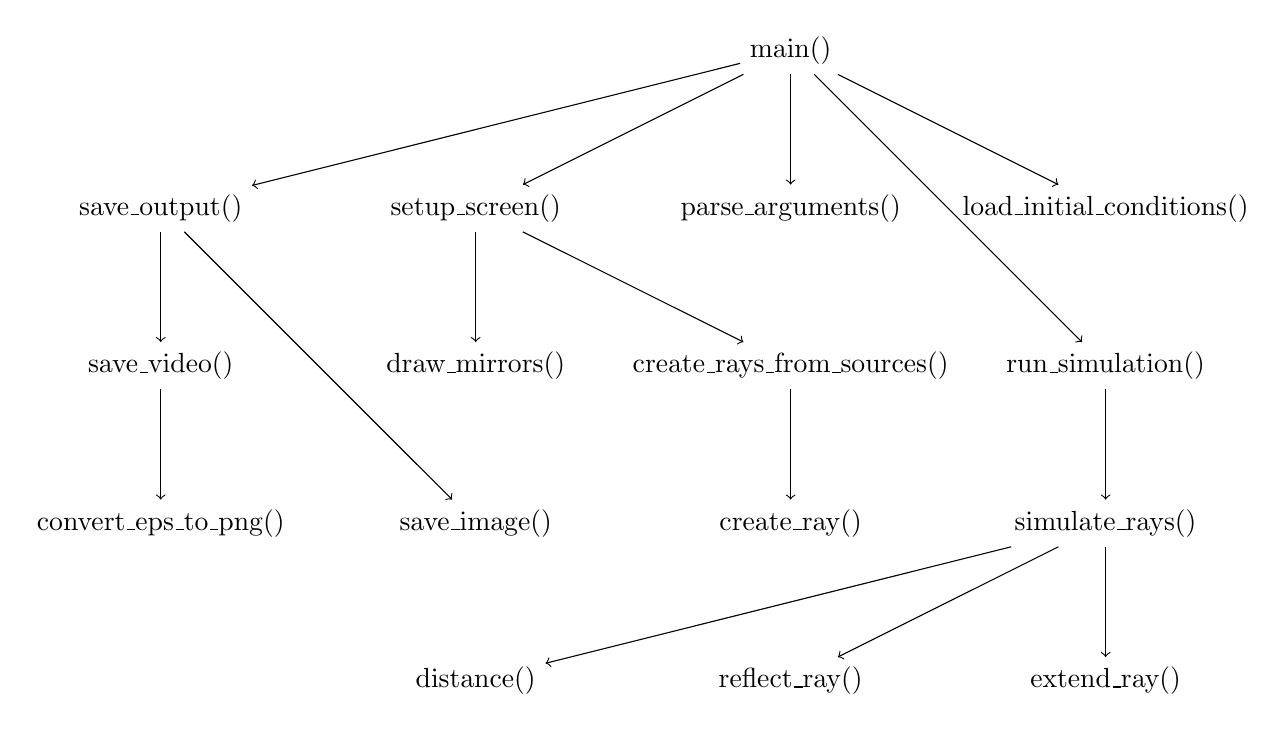
\begin{tikzpicture}[node distance=2cm, auto]
    % Nodes
    \node (main) {main()};
    \node (parse) [below of=main] {parse\_arguments()};
    \node (load) [right of=parse, xshift=2cm] {load\_initial\_conditions()};
    \node (setup) [left of=parse, xshift=-2cm] {setup\_screen()};
    \node (save) [left of=setup, xshift=-2cm] {save\_output()};
    \node (video) [below of=save] {save\_video()};
    \node (convert) [below of=video] {convert\_eps\_to\_png()};
    \node (draw) [below of=setup] {draw\_mirrors()};
    \node (image) [below of=draw] {save\_image()};
    \node (create) [right of=draw, xshift=2cm] {create\_rays\_from\_sources()};
    \node (ray) [below of=create] {create\_ray()};
    \node (run) [below of=load] {run\_simulation()};
    \node (sim) [below of=run] {simulate\_rays()};
    \node (ext) [below of=sim] {extend\_ray()};
    \node (ref) [left of=ext, xshift=-2cm] {reflect\_ray()};
    \node (dis) [left of=ref, xshift=-2cm] {distance()};

    % Arrows
    \draw [->] (main) -- (parse);
    \draw [->] (main) -- (load);
    \draw [->] (main) -- (setup);
    \draw [->] (setup) -- (draw);
    \draw [->] (setup) -- (create);
    \draw [->] (create) -- (ray);
    \draw [->] (main) -- (run);
    \draw [->] (run) -- (sim);
    \draw [->] (sim) -- (ext);
    \draw [->] (sim) -- (ref);
    \draw [->] (sim) -- (dis);
    \draw [->] (main) -- (save);
    \draw [->] (save) -- (image);
    \draw [->] (save) -- (video);
    \draw [->] (video) -- (convert);

  \end{tikzpicture}
  \caption{Flow Chart of Functions}
\end{figure}

\section{Usage Manual}

\subsection{System Requirements}
Before using the Ray Reflection Simulation, ensure that your system meets the following requirements:

\begin{itemize}
    \item Python 3.x installed
    \item Required Python libraries: Turtle, OpenCV, PIL, Rich
\end{itemize}

\subsection{Installation}

\subsubsection{Installing Python}
If Python is not already installed on your system, you can download it from the official Python website (\url{https://www.python.org/downloads/}).

\subsubsection{Installing Required Libraries}
Install the necessary Python libraries using the following command:

\begin{verbatim}
pip install turtle opencv-python pillow rich
\end{verbatim}

\subsection{Running the Simulation}

\subsubsection{Clone the Repository}
Clone the Ray Reflection Simulation repository from the project's GitHub page:

\begin{verbatim}
git clone https://github.com/salastro/reflectoray
\end{verbatim}

\subsubsection{Navigate to the Project Directory}
Enter the project directory:

\begin{verbatim}
cd ReflectoRay
\end{verbatim}

\subsubsection{Configuring the Simulation}

Edit the configuration JSON file (`initial\_conditions.json`) to define the initial conditions of the simulation. Specify mirror positions, source locations, initial angles of rays, and other parameters as needed.

The configuration file is structured as follows:

\begin{verbatim}
{
  "mirrors": [
    [[100, -100], [100, 100]],
    [[100, 100], [-100, 100]]
  ],
  "sources": [
    {"start": [0, 0], "color": "black"},
    {"start": [-50, 50], "color": "red"}
  ],
  "angles": {
    "start": 0,
    "end": 360,
    "step": 10
  },
  "iterations": 100
}
\end{verbatim}

The `mirrors` array contains the coordinates of the endpoints of each mirror. Each mirror is represented as a list of two points, where each point is a list of two numbers representing the $x$ and $y$ coordinates of the point.

The `sources` array contains the coordinates of the starting points of each ray.
Each ray is represented as a dictionary with two keys: `start` and `color`. The
`start` key contains a list of two numbers representing the $x$ and $y$
coordinates of the starting point of the ray. The `color` key contains a string
representing the color of the ray, which can be any well-known color name or a
hexadecimal color code.

The `angles` dictionary contains the starting angle, ending angle, and step size
for the rays. The `start` key contains a number representing the starting angle
of the rays. The `end` key contains a number representing the ending angle of
the rays. The `step` key contains a number representing the step size between
each ray.

The `iterations` key contains a number representing the number of iterations to
run the simulation for.

\subsubsection{Run the Simulation}

Execute the following command to run the simulation:

\begin{verbatim}
python reflectoray.py
\end{verbatim}

Help information can be displayed by passing the `--help` flag to the command:

\begin{verbatim}
python reflectoray.py --help
\end{verbatim}

which will display the following output:

\begin{verbatim}
usage: reflectoray.py [-h] [-i [IMAGE]] [-v [VIDEO]] [initial_conditions]

Ray Reflection Simulation

positional arguments:
  initial_conditions    Path to the initial conditions file (default:
                        initial_conditions.json)

options:
  -h, --help            show this help message and exit
  -i [IMAGE], --image [IMAGE]
                        Save the simulation as a png image
  -v [VIDEO], --video [VIDEO]
                        Record the simulation as a video
\end{verbatim}

\subsubsection{Save the Simulation}

The simulation can be saved as a static image (PNG) or as a video (MP4). To save
the simulation as an image, pass the `--image` flag to the command:

\begin{verbatim}
python reflectoray.py --image
\end{verbatim}

To save the simulation as a video, pass the `--video` flag to the command:

\begin{verbatim}
python reflectoray.py --video
\end{verbatim}

\begin{figure}[htbp]
  \begin{center}
    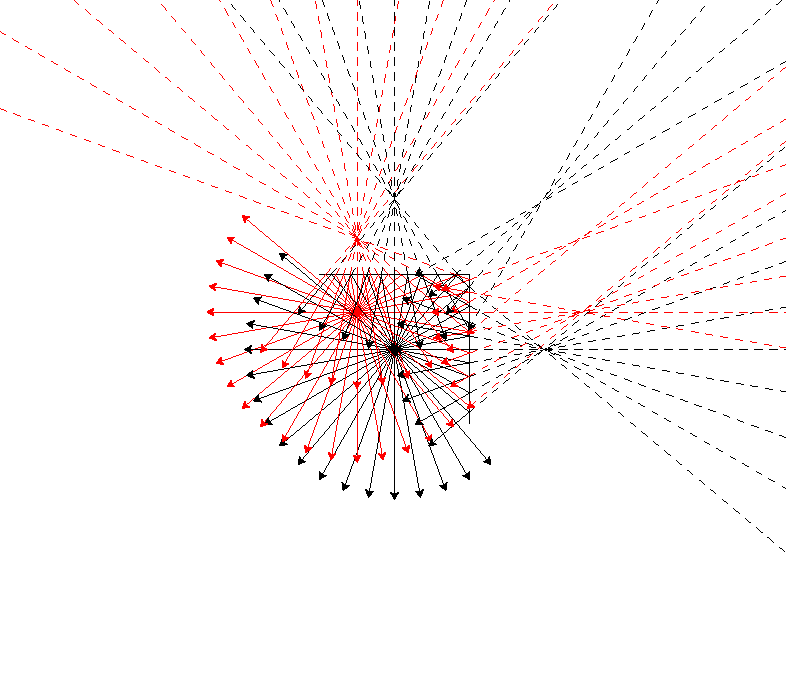
\includegraphics[width=0.95\textwidth]{figures/20231106-112653.png}
  \end{center}
  \caption{Simulation Image Output (of the default initial conditions)}
\end{figure}

\end{document}
